\section{Memorymanagement}

Es gibt verschiedene Gründe warum, nicht immer gleich viel Speicher verwendet wird z.B. da nicht unbegrenzt vorhanden ist.
Speicher wird nur dann verwendet wenn er wirklich gebraucht wird. 
Das Memorymanagement muss aktiv beachtet werden.
Es wird zwischen automatischen und manuellen Speichermanagement unterschieden. 

\subsection{Automatisch}

Automatisches Speichermanagement wird anhand der Lebenszeit einer Variable festgestellt und während dem Programmieren bereits festgelegt. 
Der Speicher liegt auf dem sogenannten \textbf{Stapel / Stack}.\\
Wird eine Funktion aufgerufen werden die benötigten Variablen auf dem Stack definiert. 
Ebenso wird eine Return Adresse zur Funktion, die die Funktion aufgerufen hat abgelegt.
Wie die Daten angeordnet werden, ist Architektur-abhängig.
Wird die Funktion wieder verlassen, werden die Variablen vom Stack wieder entfernt und zur aufrufenden Funktion zurückgesprungen.  

\subsection{Manuell/dynamisch}

Man kann auch manuell Speicher anfordern. 
Zum Beispiel, falls zur Compilezeit nicht bekannt ist wie viel Speicher gebraucht wird.
Dieser Speicher ist auf dem sogenannten \textbf{Haufen / Heap}.\\
Der Heap ist ein Speicherbereich der vom Betriebssystem bereitgestellt und verwaltet wird.\\
Zur Laufzeit wird Speicherdynamisch angefordert. 
Dieser bleibt so lange belegt bis dieser Manuell wieder freigegeben wird.\\
Es kann aber auch sein, falls der Speicher stark fragmentiert ist, das kein Speicher bereitgestellt werden kann. 
Generell ist bei sehr vollem Speicher das Arbeiten erschwert.

\subsubsection{Speicherlecks}

Falls ein Programm unkontrolliert Speicher aufnimmt oder den ihm zur Verfügung gestellte nicht wieder freigibt, spricht man von einem Speicherleck. 
Diese sind zu verhindern da diese zu einer Systemüberlastung führen und Abstürzen führen.

\subsection{Speichermanagement funktionen}

Es gibt einige Funktionen für Speichermanagement. In c und C++ sind diese leicht verschieden. 
Generell geben diese einen Pointer zurück, welcher auf freien Speicher zeigt. 
\textbf{Diese müssen immer auf einen nullpointer geprüft werden da keine garantie vorhanden ist das überhaupt speicher vorhanden ist!}
Generell sollte mit solchen Pointer immer mistrauisch gearbeitet werden und nach ambschluss immer wider freigegeben werden.

\subsubsection{C: malloc( ) calloc( ), free( ) (Funktionen)}

Malloc() gibt einen Voidpointer(pointercasting nicht vergessen) zurück welche auf eine angeforderte Grösse an Bytes Speicher zeigt. 
Der Speicher ist \textbf{nicht} initialisiert
Calloc() macht dasselbe, initialisiert aber den Speicher auf 0.\\
free() gibt den Speicherbereich wieder frei.

\lstinputlisting[language = c++]{code/mem_mngmt_c.c}

Falls kein Speicher allokiert werden kann, wird ein NULL-pointer zurückgegeben.

\subsubsection{C++: new, delete, new[ ], delete[ ] (Operatoren)}

Der New Operator erstellt ein Pointer welcher auf die mitgegebene Grösse zeigt.
new[ ] macht dasselbe, ausser das dieser ein Array zurückgibt.

Delete([ ]) gibt den Speicher wieder frei.

\lstinputlisting[language = c++]{code/mem_mngmt_cpp.cpp}

\subsection{Speicheraufbau}

Der Speicheraufbau bildlich dargestellt sieht ungefähr so aus:

\begin{center}
    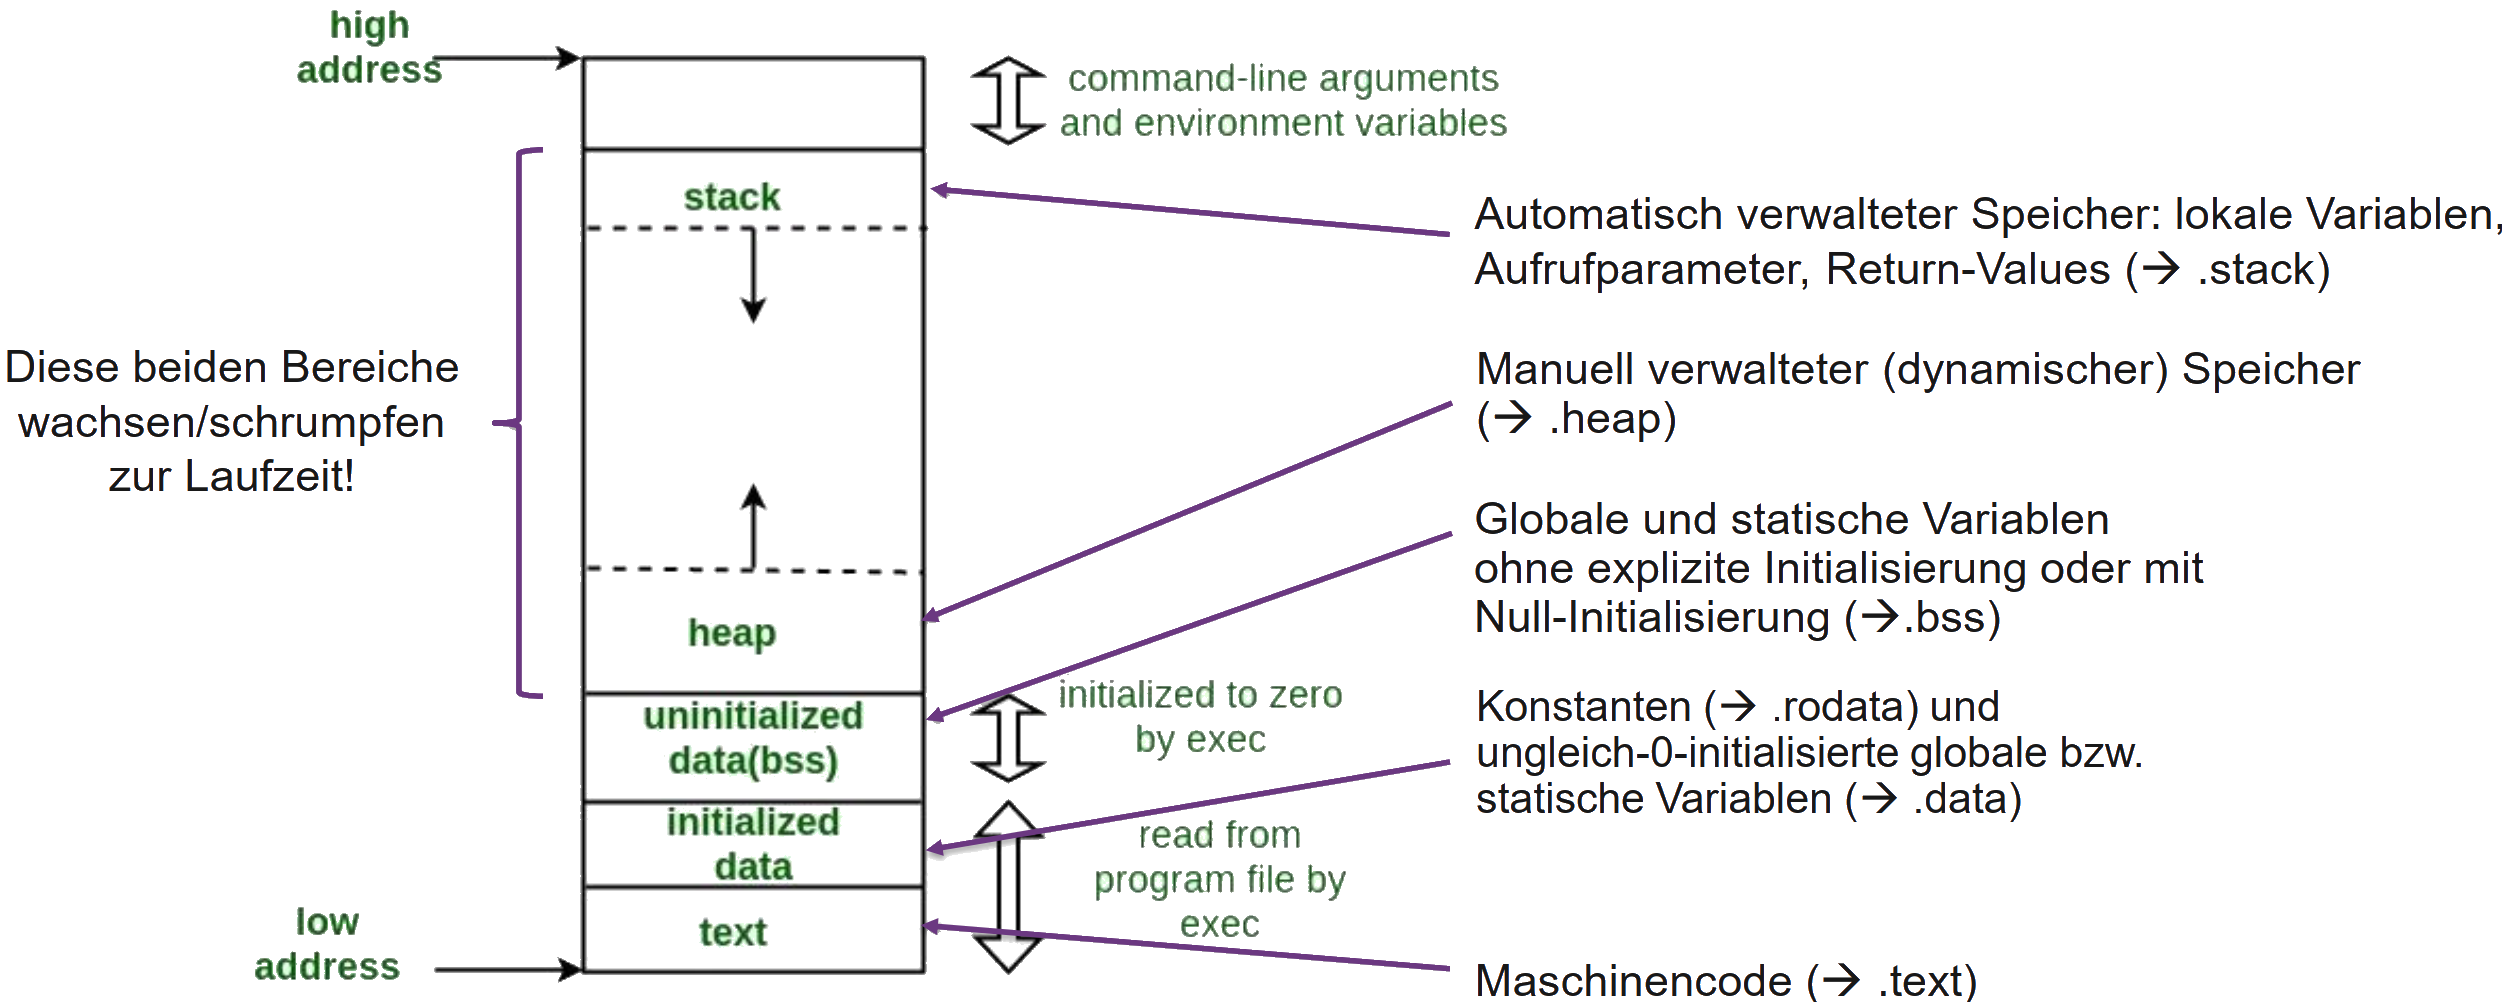
\includegraphics[width=\columnwidth]{pictures/memorylayout.png}  
\end{center}

Je nach Architektur kann es auch sein das die hohen und tiefen Adressen anders herum sind.